\documentclass[10pt,a4paper]{article}

\usepackage[abs]{overpic}
\setlength\unitlength{1mm}
\usepackage{framed, color}


\setlength\parindent{0pt}


\newlength\Li \newlength\Lii 
\setlength\Li{60mm} \setlength\Lii{80mm} 

\setlength\topmargin{-1in}
\setlength\headheight{0pt}
\setlength\headsep\headheight
\setlength\textheight\paperheight
\addtolength\textheight{-2\footskip}
\setlength\textwidth{150mm}
\setlength\oddsidemargin\paperwidth
\addtolength\oddsidemargin{-\textwidth}
\setlength\oddsidemargin{.5\oddsidemargin}
\addtolength\oddsidemargin{-1in}
\setlength\evensidemargin\oddsidemargin

\newcommand\HFILL{\hspace*{\fill}}
\newcommand\VFILL{\vspace*{\fill}}

\pagestyle{empty}

\begin{document}

\VFILL

\section*{Verwendung der \texttt{overpic} environment mit
  absoluter Positionierung}

\HFILL
\begin{minipage}{\Li}
  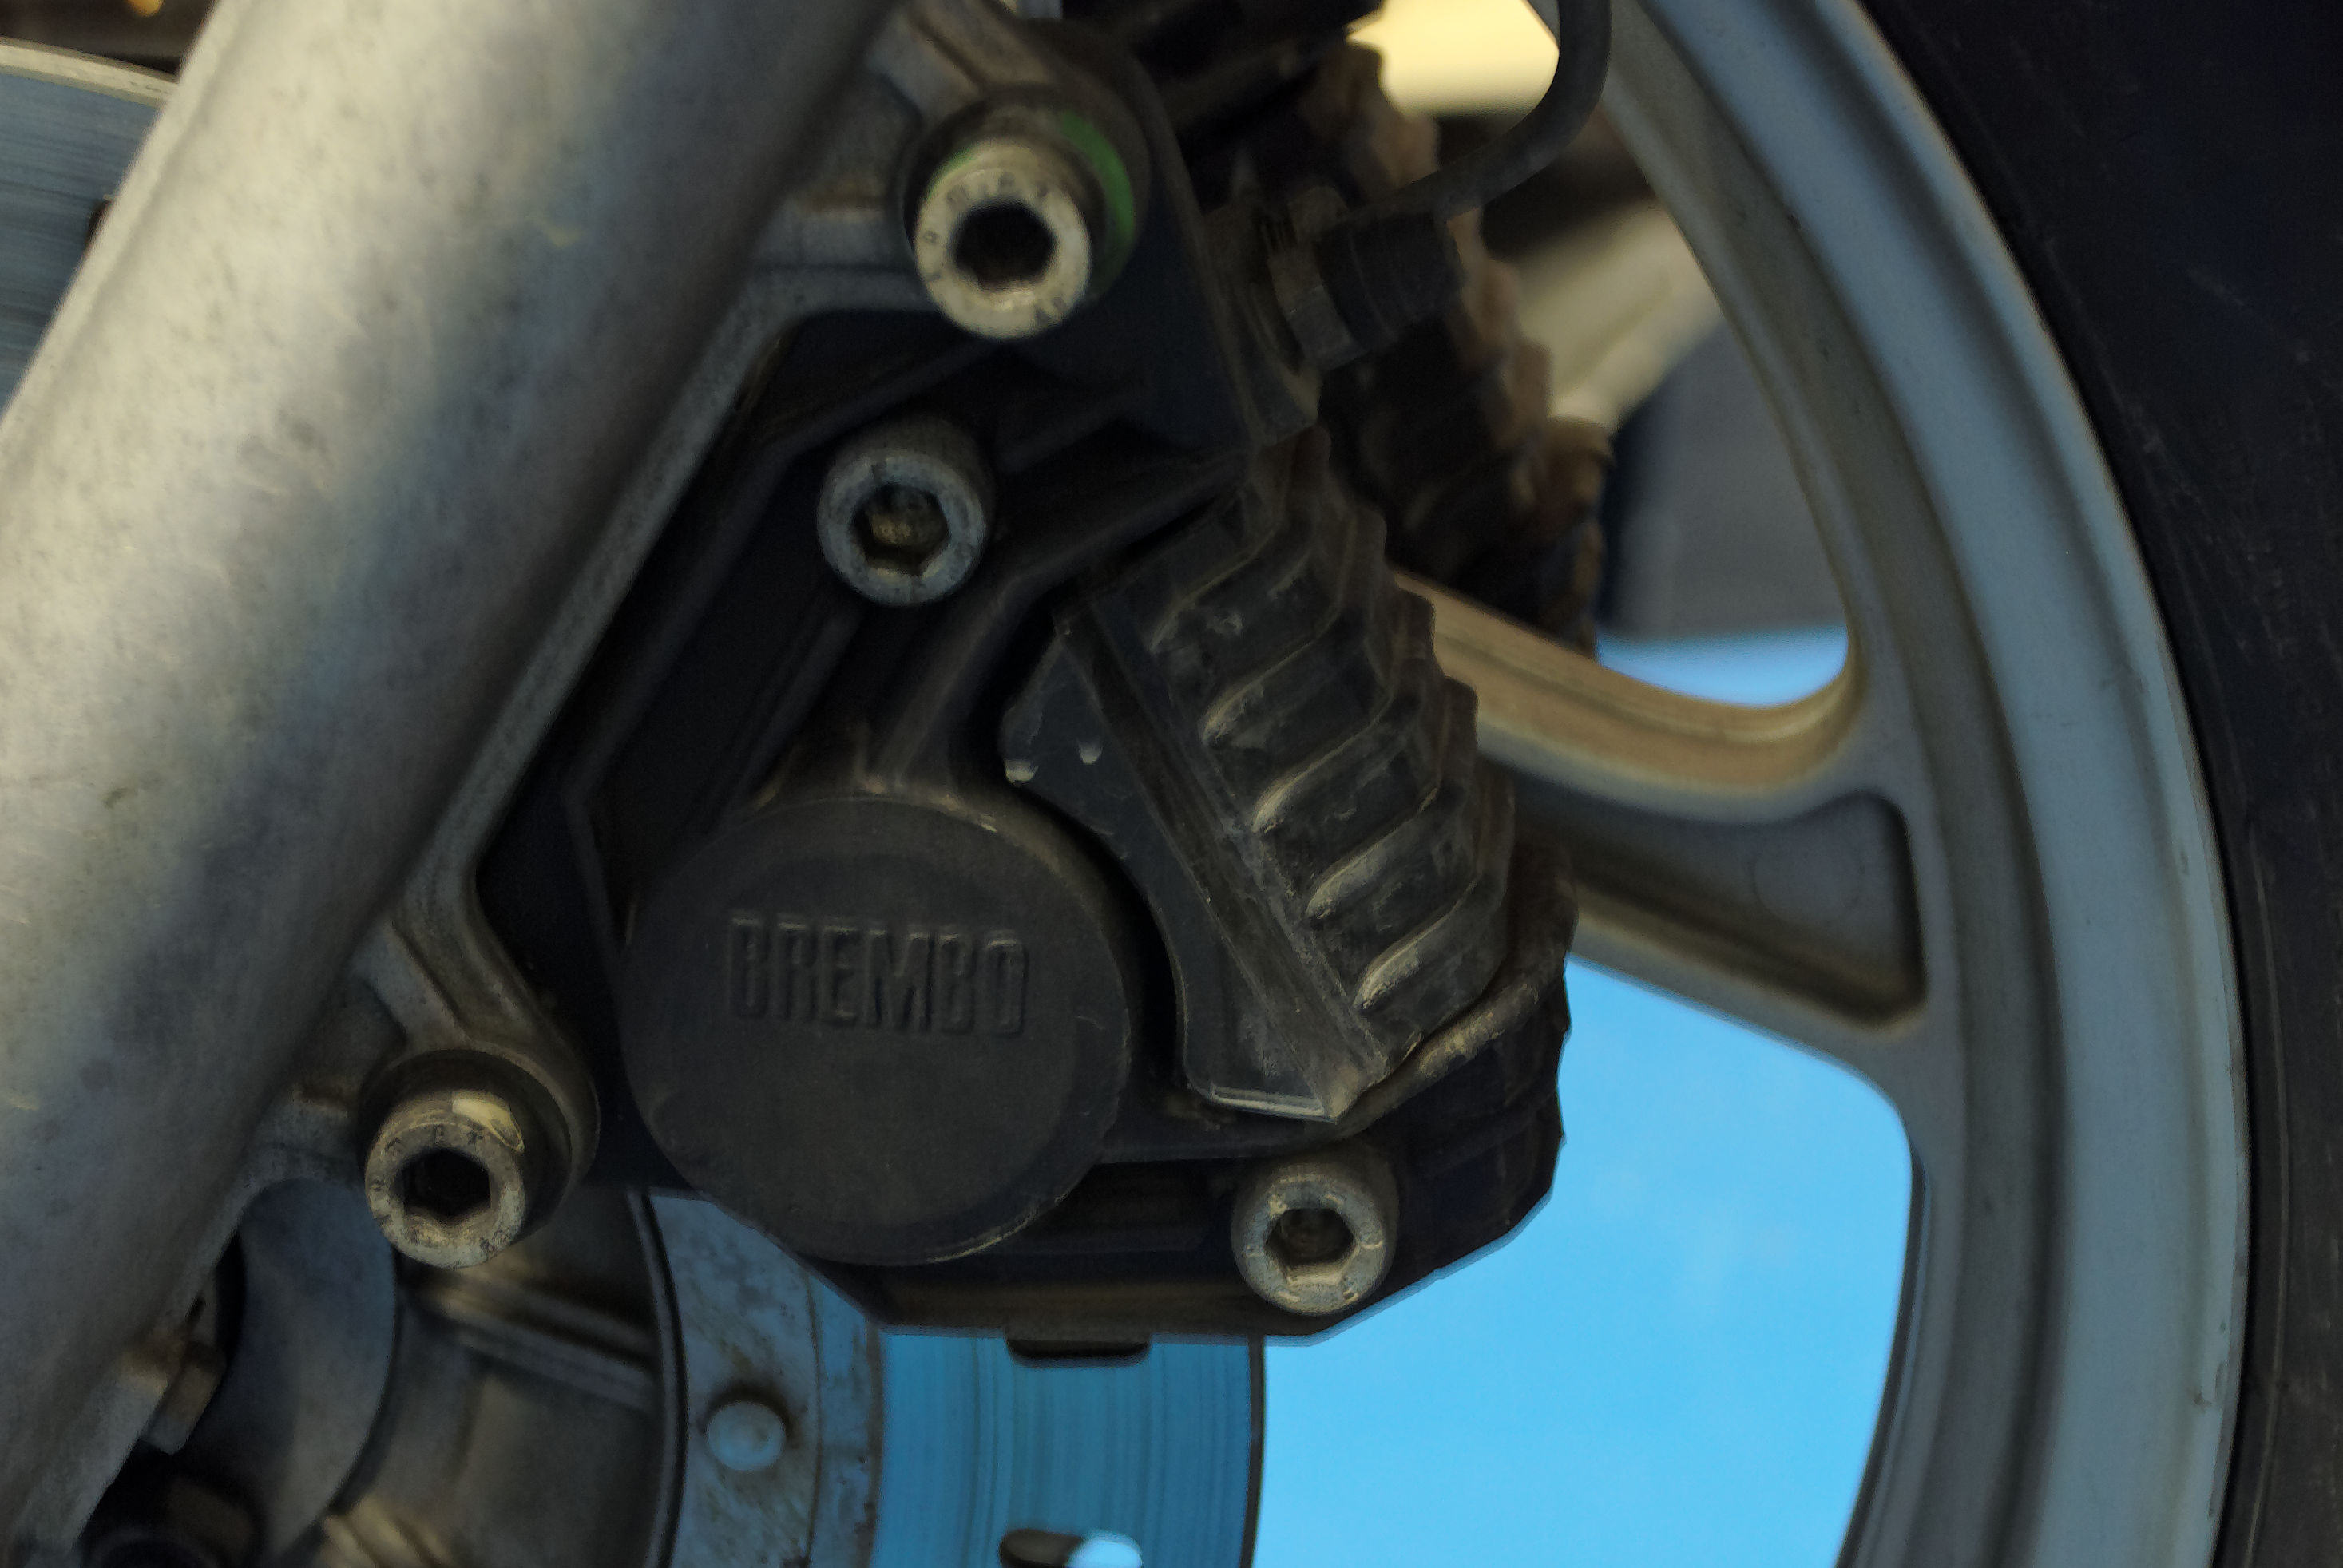
\includegraphics[width=\linewidth]{vorderrad_bremse}
\end{minipage}\qquad
\begin{minipage}{\Lii}
  Insert before:
  \begin{verbatim}
\usepackage[abs]{overpic}
...
\setlength\unitlength{1mm}
and/or local option unit=...

\usepackage{framed, color}

  \end{verbatim}    
  The  original graphic from \textsc{GhostScript}:
  \begin{verbatim}
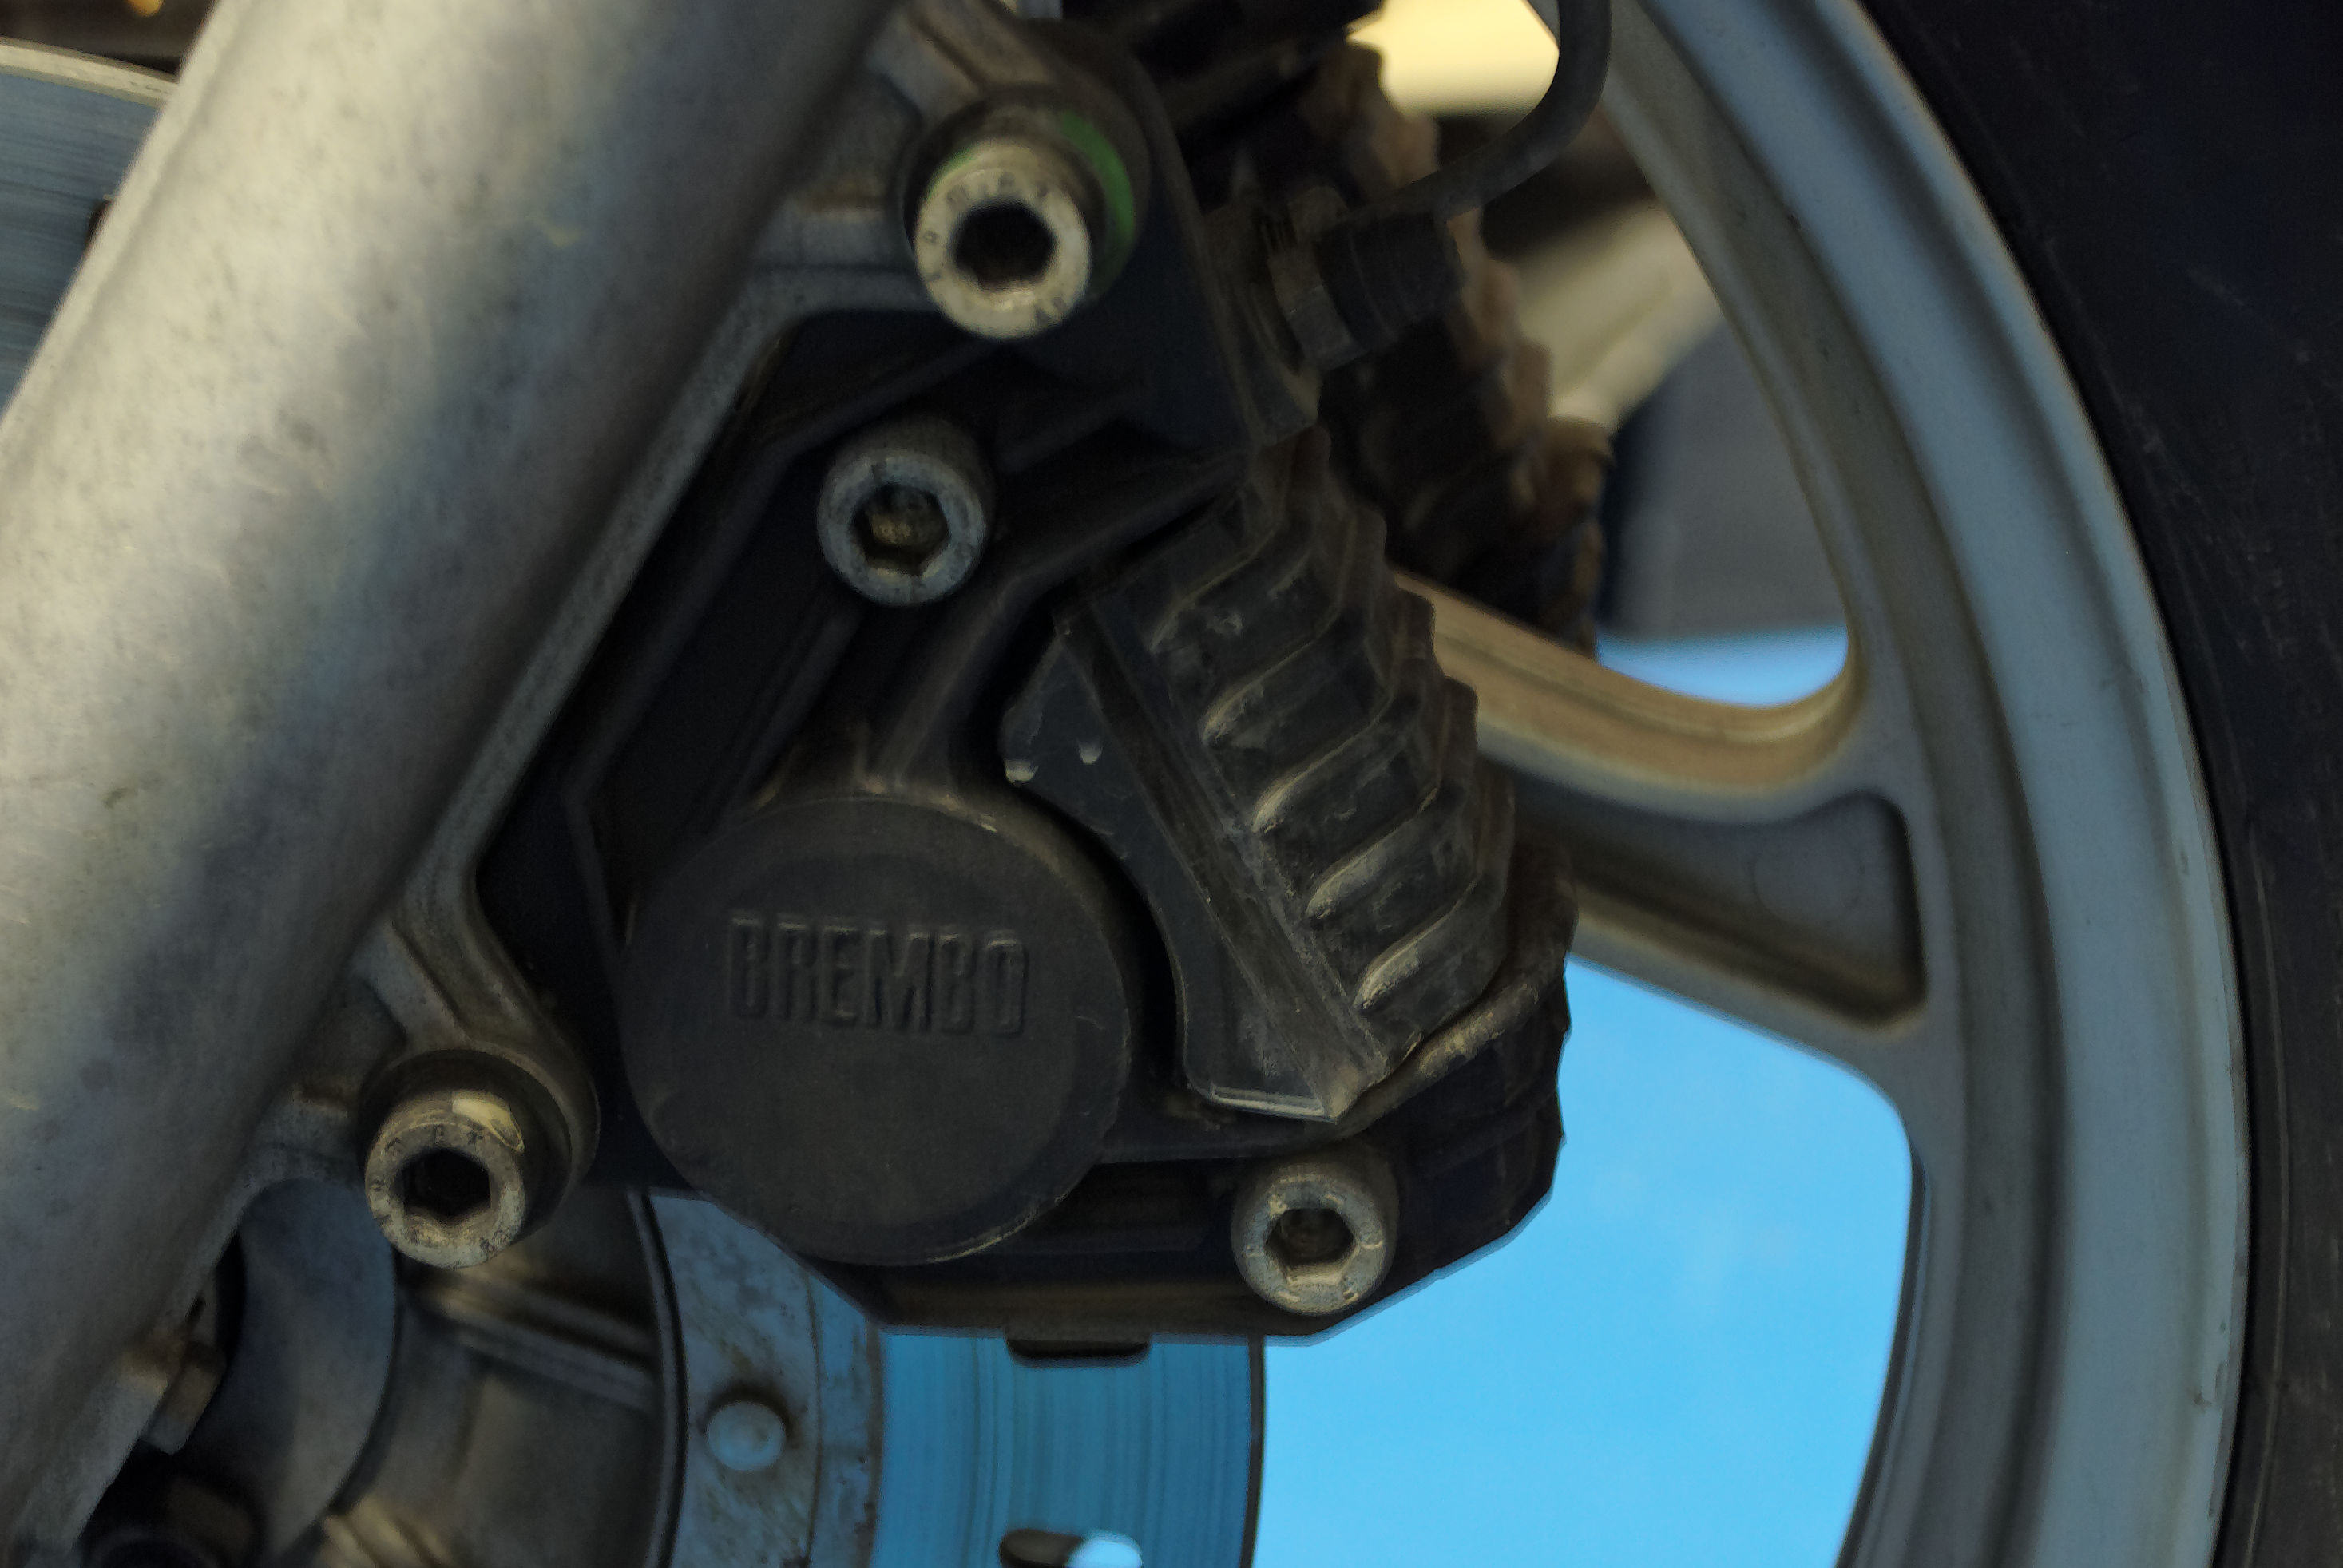
\includegraphics[width=\linewidth]{vorderrad_bremse}
  \end{verbatim}  
\end{minipage}
\HFILL

\VFILL

\HFILL
\begin{minipage}{\Li}
  \begin{overpic}[width=\linewidth,grid,tics=5]{vorderrad_bremse}
  \end{overpic}  
\end{minipage}\qquad
\begin{minipage}{\Lii}
  A grid for orientation:%  
  \begin{verbatim}
\begin{overpic}[width=\linewidth,grid,tics=5]%
      {vorderrad_bremse}
\end{overpic}
  \end{verbatim}  
  (default for \texttt{tics} is 10)  
\end{minipage}
\HFILL

\VFILL

\HFILL
\begin{minipage}{\Li}
  \begin{overpic}[width=\linewidth,unit=1mm]{vorderrad_bremse}
	\thicklines
  	\put(2,2){\vector(1,1){10}}
  	\put(5,5){\textcolor{white}{Text}}
    \put(29,33){\colorbox{white}{Inbus 1}}
    \put(14.5,9){\colorbox{white}{Inbus 2}}
  \end{overpic}  
\end{minipage}\qquad
\begin{minipage}{\Lii}
  Positioning the \LaTeX\ output with \verb#\put# commands:  
  \begin{verbatim}
\begin{overpic}[width=\linewidth,unit=1mm]%
      {vorderrad_bremse}
    \put(29,33){\colorbox{white}{Inbus 1}}
    \put(14.5,9){\colorbox{white}{Inbus 2}}
    % Weitere Möglichkeiten:
    %\put(3,28){Noch ein Text}
    %\put(3,28){\circle{2}}
    %\put(34,5){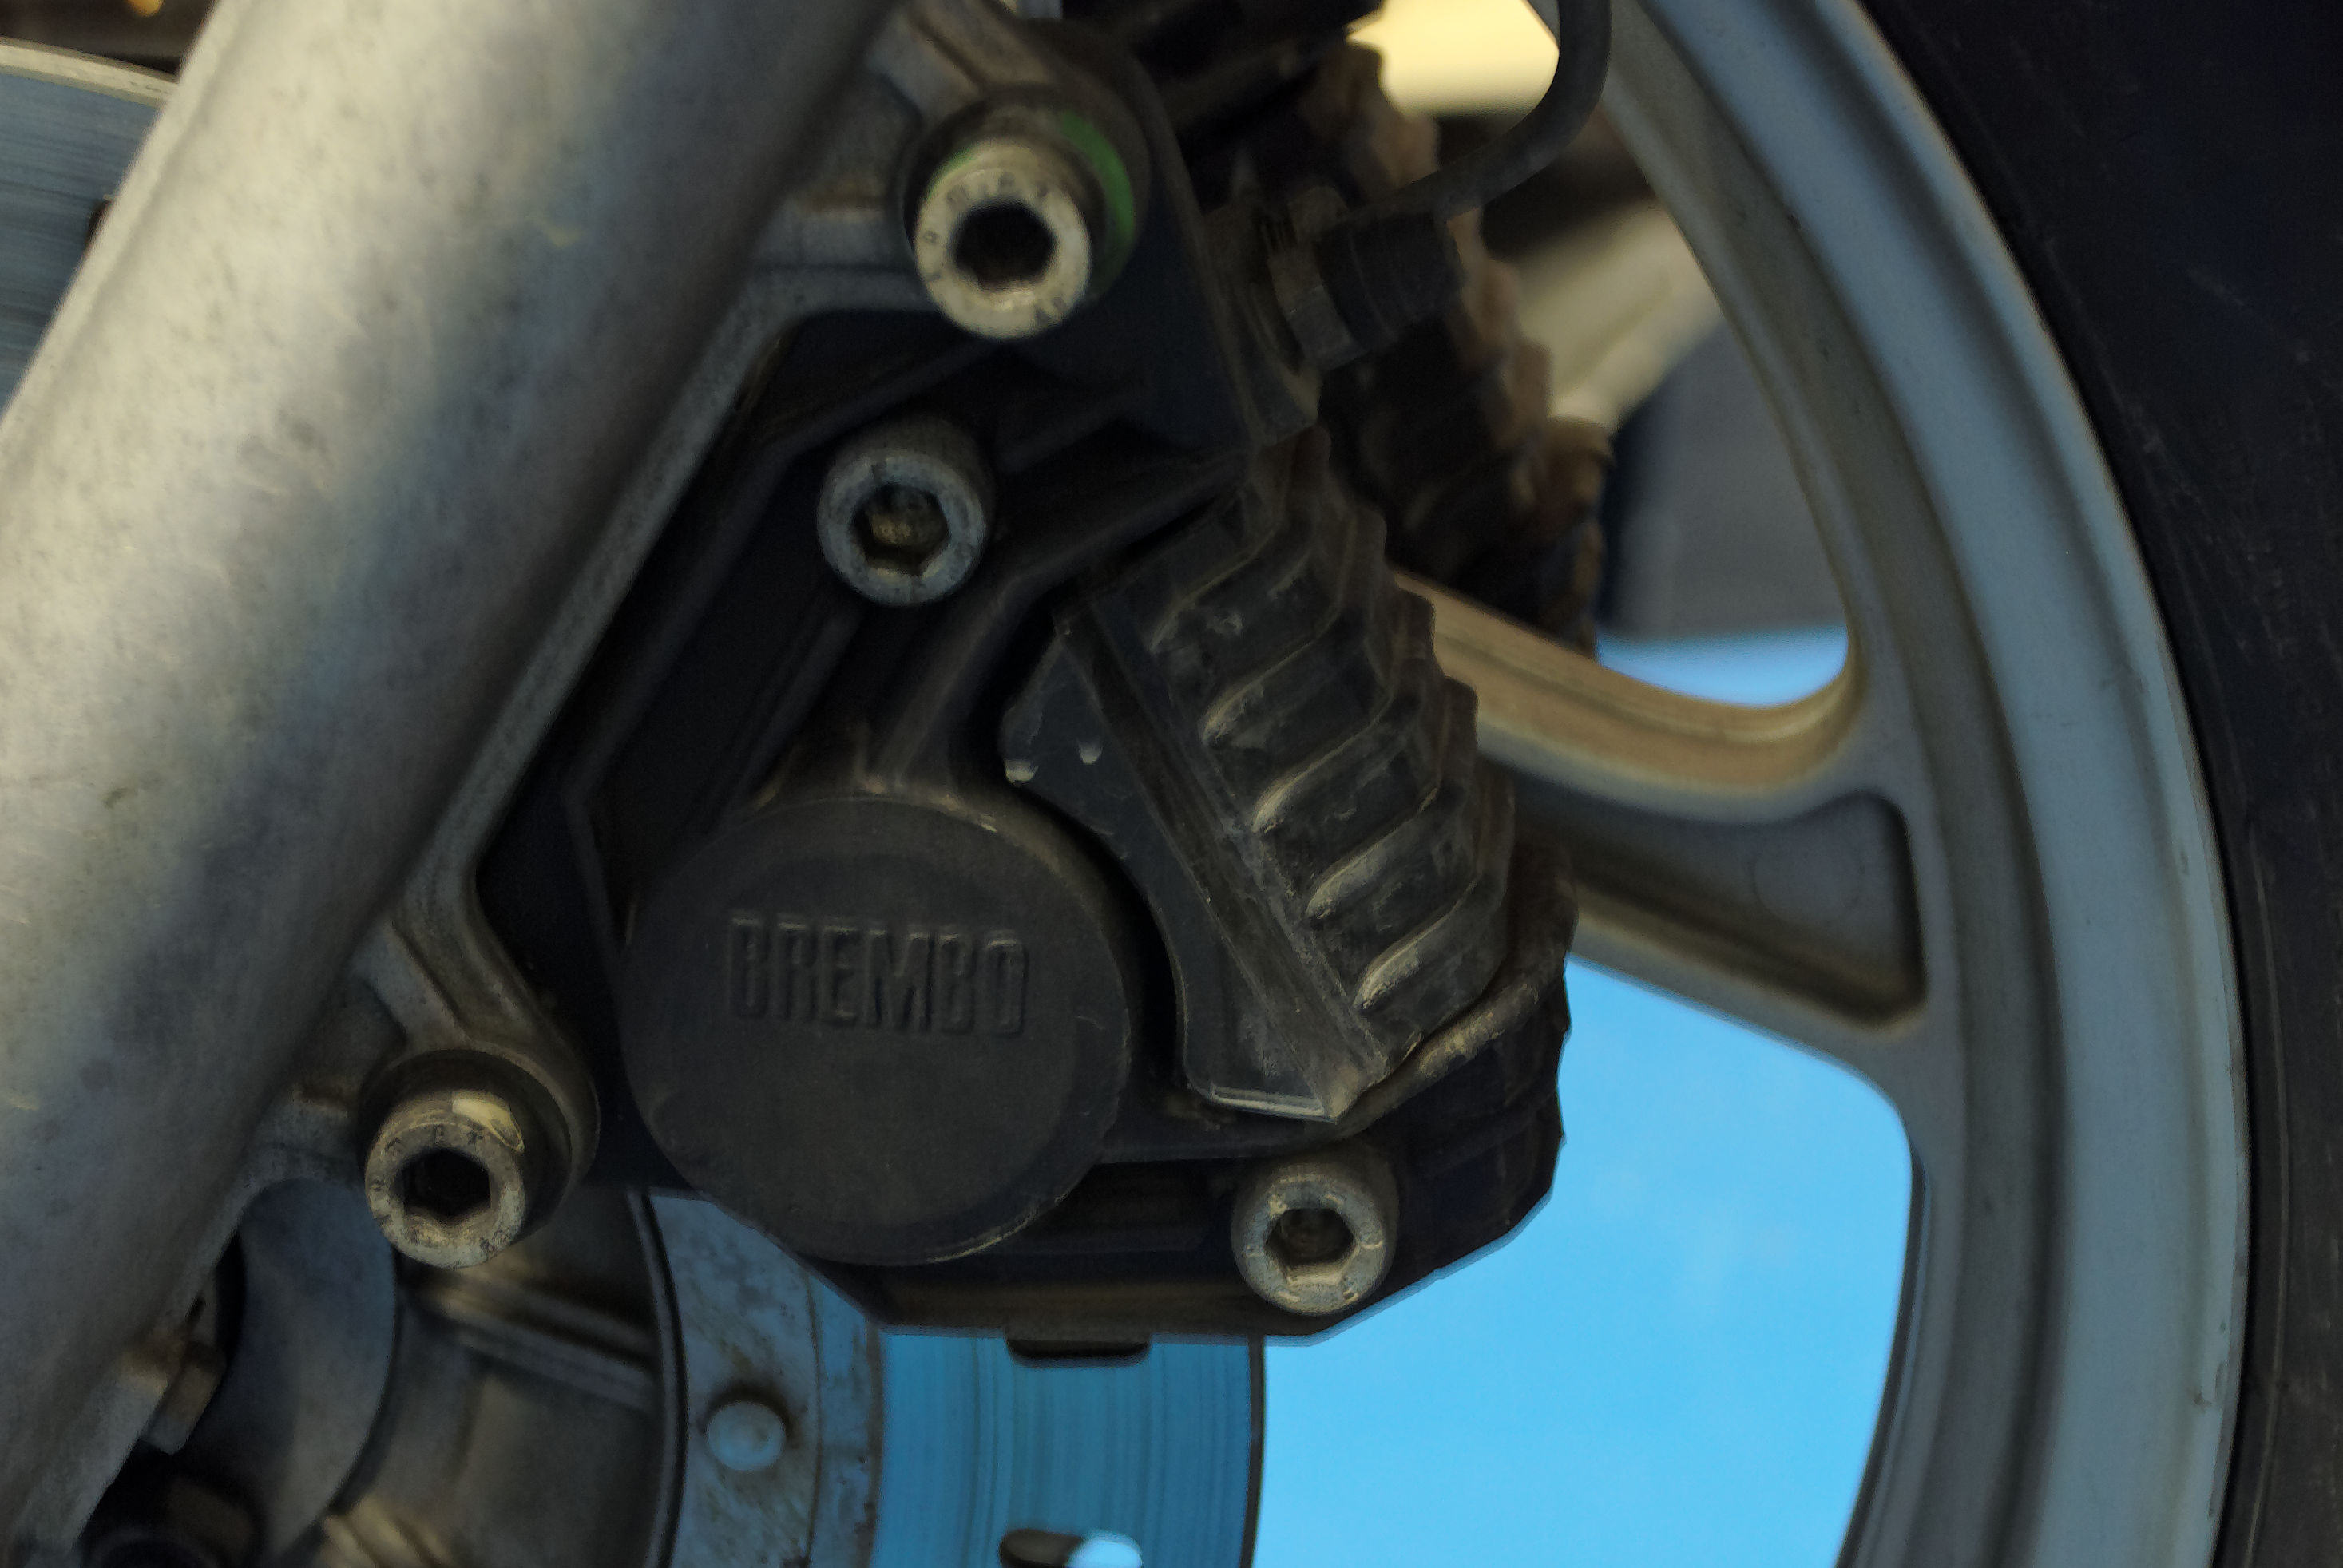
\includegraphics[scale=.07]{vorderrad_bremse}}
\end{overpic}
  \end{verbatim}
  (default for \texttt{unit} is \verb#\unitlength#)  
\end{minipage}
\HFILL

\VFILL

\end{document}
